\documentclass[11pt]{article}

\usepackage[margin=1.1in]{geometry}
\usepackage[T1]{fontenc}
\usepackage[utf8]{inputenc}
\usepackage{newtxtext,newtxmath}
\usepackage{microtype}
\usepackage{graphicx}
\usepackage{booktabs}
\usepackage{amsmath}
\usepackage{xcolor}
\usepackage[round,authoryear]{natbib}
\usepackage{caption}
\usepackage[colorlinks=true,linkcolor=blue!60!black,citecolor=blue!60!black,urlcolor=blue!60!black]{hyperref}

\captionsetup{font=small,labelfont=bf}
\graphicspath{{figures/}}

\newcommand{\judgemode}[1]{\texttt{#1}}
\newcommand{\repourl}{https://github.com/AbdelStark/leworldmodel-judge}
\newcommand{\datasetsurl}{https://huggingface.co/datasets/abdelstark/leworldmodel-judge-runs}

\title{A World Model as a Judge: Early, Auditable Verdicts\\on Partial Robot-Manipulation Rollouts}

\author{%
  Abdelhamid Bakhta\\
  StarkWare\\
  \texttt{abdel@starkware.co}%
}

\date{July 13, 2026\\[0.4em]
\small Companion paper to \texttt{leworldmodel-judge} v0.2.0\thanks{Code, benchmark
artifacts, and reproduction commands: \url{https://github.com/AbdelStark/leworldmodel-judge}.
Published cloud runs with full provenance: \url{https://huggingface.co/datasets/abdelstark/leworldmodel-judge-runs}.}}

\begin{document}

\maketitle

\begin{abstract}
We present \textbf{LeWorldModel Judge}, a locked benchmark and an auditable judging surface
for scoring partial robot-manipulation rollouts before their episodes end. Sparse terminal
reward answers no useful question about a trajectory prefix: whether the rollout is still on
track, already doomed, or physically implausible only becomes visible in hindsight, which
makes early triage, data curation, and process-reward experiments needlessly blind. We lock a
narrow evaluation slice (three Meta-World tasks, four constructed policy families, prefix
cutoffs at 0.25, 0.50, and 0.75 of the horizon), define heuristic but fully inspectable
prefix labels, and score every prefix with a cutoff-time composite judge over named evidence
signals, alongside a replay-time latent proxy whose causal limitation we state exactly. A
mandatory calibration protocol reports the provenance of every decision threshold and only
grants held-out status when the calibration and evaluation policy families are disjoint.
On a fresh 90-prefix held-out slice collected after the label rules were frozen, the
composite judge reaches a 0.949 failure hit rate at a 0.137 false positive rate and 0.978
pairwise ranking accuracy, against 0.50 and 0.554 for sparse-reward and progress baselines,
and the threshold calibrated on disjoint families transfers across disjoint captures to
within 0.0004 (0.2977 versus 0.2980). Every reported number decomposes to named sub-scores in
checked-in files, carries a \judgemode{judge\_mode} provenance tag, and regenerates from a
pinned command line.
\end{abstract}

\section{Introduction}
\label{sec:intro}

A sparse success signal is silent until it is too late. In manipulation benchmarks the reward
that matters is terminal: the object ends in place or it does not, and until that moment the
learner, the operator, and any data-curation pipeline sitting between them are equally
uninformed. Yet most of the questions practitioners actually ask concern the middle of a
rollout. Is this trajectory still likely to succeed? Has it already become unrecoverable?
Does the state evolution look physically wrong? How much should we trust any of those calls?

This paper describes a deliberately narrow system that answers those questions on a locked
benchmark slice and, just as deliberately, refuses to answer anything wider. The project is
anchored in the world-model research program associated with joint-embedding predictive
architectures \citep{lecun2022path, assran2023ijepa, bardes2024vjepa}: a world model that
predicts how an episode should continue supplies a natural surprise signal for judging how an
episode is actually going. The shipped implementation, however, is not a trained world model,
and we do not present it as one. It is a hand-weighted composite over decomposed prefix
evidence plus a linear observation-space proxy, and the distinction between the conceptual
anchor and the shipped mechanism is maintained everywhere, including in the per-row
provenance tags of the released data.

The contribution is best read as a benchmark-and-protocol result rather than a modeling
result:

\begin{itemize}
  \item \textbf{A locked benchmark for prefix-level trajectory verification.} Three
  Meta-World tasks \citep{yu2020metaworld}, four constructed policy families (expert, weak,
  doomed, misleading), prefix cutoffs at fractions 0.25, 0.50, and 0.75 of the episode
  horizon, heuristic task-aware failure and recoverability labels, and a fixed baseline set.
  The slice is small by design: every claim in this paper traces to files small enough to
  read.
  \item \textbf{An auditable judging surface.} Every verdict is serialized with the seven
  named evidence fields of the record contract, joined by key to the prefix record that holds
  the remaining raw inputs, every row carries a \judgemode{judge\_mode} tag naming the
  implementation that produced it, and a null judge with the same record shape sanity-checks
  the harness. The composite judge is cutoff-time: it reads nothing past the
  cutoff. A hybrid variant that consumes a latent proxy is replay-time by construction, and
  we treat that causal boundary as part of the result rather than a footnote.
  \item \textbf{A calibration protocol with mandatory provenance.} Every reported threshold
  states whether it was fixed in advance, tuned in-slice, or calibrated on a held-out family
  split, and held-out status is only granted when calibration and evaluation families are
  disjoint. Reviewer-facing summaries name the cohorts and their label counts.
  \item \textbf{Evidence that the protocol does useful work.} On the initial 18-prefix
  held-out slice the judge separates perfectly, which proves wiring rather than
  generalization. On a fresh capture collected after the label rules were frozen, with five
  times the evaluation cohort, perfect separation degrades honestly (hit rate 0.949, false
  positive rate 0.137) while the ranking gap over sparse-reward and progress baselines
  persists (0.978 versus 0.50 and 0.554), and the calibrated operating point transfers across
  disjoint captures to within 0.0004.
\end{itemize}

We also report the negative and confounded results with the same prominence. No episode in
either real capture reaches terminal success within the 75-step cap, so on real data every
detection metric rests on the heuristic prefix labels rather than environment truth. The
labeler and the judge draw on the same evidence family, and a single shared feature (distance
regret) achieves 0.824 pairwise accuracy on the fresh held-out slice against the judge's
0.978, which bounds how much of the ranking signal is attributable to the composite rather
than to its strongest input. Section~\ref{sec:limitations} discusses both issues.

\section{Related work}
\label{sec:related}

\paragraph{World models and predictive representations.}
Learning a model of environment dynamics and using its predictions as a training or planning
substrate is a long-standing program \citep{ha2018worldmodels, hafner2020dreamer,
hafner2023dreamerv3, hansen2022tdmpc}. Joint-embedding predictive architectures move
prediction into representation space: predict the embedding of a missing view rather than
its pixels, whether masked regions of the same image \citep{assran2023ijepa}, masked
spatio-temporal regions of a video \citep{bardes2024vjepa}, or, in the proposed full
architecture, future world states \citep{lecun2022path}. Our work borrows the judging
intuition from this line (a predictor's disagreement with reality is evidence about the
trajectory) without yet training a predictor; the shipped latent proxy is a linear
extrapolation over mean-pooled observation windows, and we label it as such.

\paragraph{Surprise as a signal.}
Prediction error has served as an intrinsic reward for exploration \citep{pathak2017curiosity,
burda2019rnd} and as an ensemble-disagreement objective for model-based exploration
\citep{sekar2020plan2explore}. We invert the sign of the argument: rather than seeking
surprising states, we ask whether a partial rollout is consistent with a predicted successful
continuation, and treat inconsistency as evidence of failure.

\paragraph{Verifiers and process reward models.}
Outcome-supervised verifiers rerank candidate solutions by predicted correctness
\citep{cobbe2021verifiers}, and process supervision scores intermediate steps rather than
final answers \citep{uesato2022process, lightman2024verify}. Preference-based reward models
occupy the same trust-critical position in RLHF pipelines \citep{christiano2017preferences}.
Our judge is the embodied analogue of a process reward signal, with one additional design
constraint these lines rarely impose: every score must decompose into inspectable evidence
so that a skeptical reviewer can challenge an individual verdict without rerunning anything.

\paragraph{Failure detection in manipulation.}
Dedicated failure detectors for manipulation include multimodal sensor-fusion classifiers
\citep{inceoglu2021finonet}, vision-language success detectors \citep{du2023vlmsuccess}, and
LLM-based post-hoc failure explanation \citep{liu2023reflect}. These systems mostly classify
completed or nearly completed executions; our benchmark targets the earlier question of what
can be said at fixed fractional cutoffs of a still-running episode, and evaluates ranking as
well as detection.

\paragraph{Evaluating without executing.}
Off-policy evaluation estimates policy value from logged data \citep{thomas2016hcope,
levine2020offline}. Prefix judging is a complementary, more granular problem: not the value
of a policy, but the fate of one partially observed trajectory. We use standard
threshold-free ranking statistics precisely because operating points chosen on the evaluation
slice are the classic failure mode of such comparisons.

\section{The benchmark}
\label{sec:benchmark}

\subsection{Environment slice and policy families}

The benchmark locks three Meta-World tasks \citep{yu2020metaworld} on MuJoCo physics
\citep{todorov2012mujoco} behind the Gymnasium interface \citep{towers2024gymnasium}:
\texttt{reach-v3}, \texttt{push-v3}, and \texttt{pick-place-v3}. Rollouts come from scripted
expert policies degraded per \emph{policy family}, so that failure modes exist by
construction rather than by accident:

\begin{itemize}
  \item \textbf{expert}: the scripted policy, unmodified;
  \item \textbf{weak}: actions scaled to 0.55 of expert magnitude with shared-scalar noise on
  the translation dimensions;
  \item \textbf{doomed}: expert actions negated and rescaled after 40\% of the horizon;
  \item \textbf{misleading}: expert behavior that switches to zero actions after 30\% of the
  horizon, so early evidence looks healthy and late evidence is dead.
\end{itemize}

A fifth family (\textbf{random}) exists in the collector as a negative control and is not
part of the reported slices. Episodes are captured at up to 75 steps; a capture is 5 episodes
per (task, family) pair in the fresh run reported here (60 episodes, 4{,}500 step records) and
1 episode per pair in the initial capture (12 episodes). Meta-World physics is not
byte-reproducible across simulator builds, so each capture's \texttt{rollouts.jsonl} is
checked in as the input of record and everything downstream regenerates deterministically
from it.

\subsection{Prefixes, labels, and what the labels are not}
\label{sec:labels}

Each episode is sliced at fractional cutoffs $f \in \{0.25, 0.50, 0.75\}$ of its realized
horizon. A prefix record carries the evidence signals available up to the cutoff, derived
from Meta-World info fields: distance progress and its decomposition (start, best, and last
distance to target), an in-place score, near-object and grasp signal peaks, a success signal
peak, reward density (mean non-negative unscaled reward), a stall score, and a progress
proxy. Missing signals remain \texttt{null}; absence is never coerced to zero.

Each prefix receives two labels from a task-aware heuristic labeler:
\texttt{prefix\_failure\_label} (boolean: effectively doomed at this cutoff) and
\texttt{prefix\_recoverability\_label} (recoverable, at risk, or doomed). The rules are
deliberately conservative: episodes that end in success are never failure-labeled, a prefix
with no observed state signal is at most at risk, and no prefix is labeled doomed before
cutoff 0.5. Task-specific gates handle the ways each task actually dies; the
\texttt{push-v3} gates were hardened against noisy contact signals masking dead trajectories.

Two properties of these labels matter for interpreting every number that follows. First,
they are heuristics over the same evidence family the judge reads, not independent ground
truth; only \texttt{final\_success\_label} is environment truth, and it only vetoes failure
labels on successful episodes. Second, in both real captures reported here, no episode
reaches terminal success within the 75-step cap, so the veto never fires and the real-data
metrics rest entirely on the heuristic labels. We measure the practical consequence of this
circularity in Section~\ref{sec:circularity} rather than asking the reader to take it on
faith.

\subsection{Baselines, metrics, and calibration protocol}
\label{sec:protocol}

Every prefix is scored by three baselines on the same records as the judge: cumulative
sparse reward over the prefix (absence of reward read as predicted failure), a progress
proxy against a fixed threshold of 0.2, and terminal success, which is excluded from the
comparison as an oracle upper bound because it is not available at the cutoff.

Reported metrics per slice: failure hit rate (fraction of failure-labeled prefixes flagged),
false positive rate, pairwise ranking accuracy (the probability that a uniformly drawn
failure-labeled prefix outscores a uniformly drawn unlabeled one, ties counted half, which
equals AUROC), and average precision. Metrics pool the three cutoffs; per-cutoff detection
lead time is future work and we do not claim it.

The failure threshold applied to the judge must state its provenance in every summary file:
\emph{fixed} (chosen before looking at the slice), \emph{in-slice} (tuned by balanced
accuracy on the reported slice; a debugging operating point, never a deployment claim), or
\emph{held-out} (\texttt{held\_out\_family\_split}: tuned on a calibration cohort of policy
families disjoint from the evaluation families). The evaluator refuses to emit held-out
provenance when the family sets overlap. Baselines are deliberately not calibrated; the
false positive row therefore compares a calibrated judge operating point against
uncalibrated baseline defaults, and the threshold-free ranking rows carry the
calibration-fair comparison.

\section{The judge}
\label{sec:judge}

\subsection{Output contract}

For a prefix with evidence vector $E$, a judge emits four scores in $[0,1]$:
\texttt{on\_track}, \texttt{failure}, \texttt{implausibility}, and \texttt{uncertainty},
together with seven named evidence fields (progress, distance progress, in-place,
near-object, grasp, reward, stall) and a \judgemode{judge\_mode} tag naming the
implementation. The remaining raw inputs, including the target distances behind the
distance-regret term and the success signal peak, live in the prefix record checked in
beside the judge rows and joined by the same key; auditing a verdict end to end reads the
pair, not the judge row alone. A null judge (all scores zero,
uncertainty one) shares the record shape so the harness can be checked against a signal-free
scorer. The judge never reads the labels; a regression test pins that flipping every label
leaves every score unchanged.

\subsection{Composite cutoff-time judge}
\label{sec:composite}

The headline judge (\judgemode{composite\_prefix\_judge}) derives intermediate features from
the evidence: target proximity, distance regret (how far the object has drifted back from
its best distance), engagement (near-object or grasp), transport (in-place, success, or
distance progress), early patience (engaged early prefixes are forgiven), stalling without
transport, and engagement without transport. The failure score is a hand-weighted linear
combination of these features clipped to $[0,1]$; the weights are frozen constants in the
released code, and we make no claim that they are optimal. What we do claim is the causal
property: the composite judge reads only prefix evidence, so its verdict is computable on a
live rollout at the moment of the cutoff.

\subsection{Latent proxy and the replay-time boundary}
\label{sec:latent}

The hybrid judge (\judgemode{hybrid\_prefix\_latent\_judge}) adds a surprise term derived
from an intentionally simple latent cache. For an episode with observations
$o_{1:T}$ and a prefix of length $k$:
\begin{align*}
z_{\text{ctx}} &= \tfrac{1}{k}\textstyle\sum_{t \le k} o_t, \qquad
\bar{\Delta} = \tfrac{1}{k-1}\textstyle\sum_{t < k} (o_{t+1} - o_t),\\
\hat{z}_{\text{fut}} &= z_{\text{ctx}} + (T - k)\,\bar{\Delta}, \qquad
z_{\text{fut}} = \tfrac{1}{T-k}\textstyle\sum_{t > k} o_t,
\end{align*}
and the mismatch score is the mean absolute gap between $\hat{z}_{\text{fut}}$ and
$z_{\text{fut}}$, clipped to $[0,1]$. High mismatch raises the failure, implausibility, and
uncertainty scores and lowers the on-track score relative to the composite row.

This construction is an observation-space placeholder for a learned encoder, and it has a
causal asymmetry that we treat as a first-class result: $z_{\text{fut}}$ reads observations
after the cutoff, so the hybrid score exists only in replay. It is a hindsight consistency
check for completed episodes, useful for triage, and it is not an early-verdict signal. The
same standard excludes terminal success from the baseline set. On the initial held-out
capture the distinction costs nothing: the composite judge reproduces the hybrid headline
metrics exactly, with the latent term moving individual failure scores by at most $+0.036$
(mean $+0.011$). Any early-verdict claim in this paper therefore rests on the composite
judge alone.

\section{Results}
\label{sec:results}

All numbers below are read from checked-in summary files in the repository; each carries its
\judgemode{judge\_mode} and threshold provenance, and the captions name the source file. We
report three slices: the canonical synthetic benchmark, the initial real held-out capture,
and a fresh real capture collected after the label rules were frozen.

\subsection{Held-out family split on real captures}
\label{sec:heldout}

\begin{table}[t]
\centering
\small
\caption{Composite judge versus baselines under the held-out family split (calibrated on
weak and doomed families, evaluated on expert and misleading). Left: initial capture
(\texttt{hard-family-real-held-out-2026-04-28}, evaluation cohort $n{=}18$, threshold
0.298006). Right: fresh capture collected with frozen label rules
(\texttt{hard-family-real-fresh-capture-2026-07-13}, $n{=}90$, threshold 0.297680). All
judge rows are \judgemode{composite\_prefix\_judge}; pairwise accuracy equals AUROC.}
\label{tab:heldout}
\begin{tabular}{lcccccc}
\toprule
& \multicolumn{3}{c}{Initial capture ($n{=}18$)} & \multicolumn{3}{c}{Fresh capture ($n{=}90$)}\\
\cmidrule(lr){2-4}\cmidrule(lr){5-7}
Metric & Judge & Sparse & Progress & Judge & Sparse & Progress\\
\midrule
Failure hit rate $\uparrow$ & \textbf{1.000} & 1.000 & 1.000 & 0.949 & \textbf{1.000} & \textbf{1.000}\\
False positive rate $\downarrow$ & \textbf{0.100} & 1.000 & 1.000 & \textbf{0.137} & 1.000 & 1.000\\
Pairwise accuracy $\uparrow$ & \textbf{1.000} & 0.500 & 0.556 & \textbf{0.978} & 0.500 & 0.554\\
Average precision $\uparrow$ & \textbf{1.000} & 0.444 & 0.485 & \textbf{0.971} & 0.433 & 0.463\\
\bottomrule
\end{tabular}
\end{table}

Table~\ref{tab:heldout} contains the central comparison. Three observations, in decreasing
order of importance.

\textbf{The ranking gap survives a fresh capture at five times the cohort.} Both baselines
flag every prefix on these slices (their false positive rate is 1.0), so raw detection is
uninformative; the judge's value is concentrated in false positives and ranking quality. On
the fresh capture the composite judge holds 0.978 pairwise accuracy against 0.500 for sparse
reward and 0.554 for the progress proxy, and 0.971 average precision against 0.433 and
0.463 (Figure~\ref{fig:baselines}).

\textbf{The calibrated operating point transfers across captures.} Calibrating on the fresh
capture's weak and doomed cohort (90 prefixes, 32 failure-labeled) yields threshold
0.297680; the same procedure on the initial capture's 18-prefix cohort had yielded
0.298006. Disjoint episodes, seeds, and cohort sizes recover the same operating point to
within $4\times10^{-4}$ (Figure~\ref{fig:transfer}). We did not expect agreement this tight
and make no claim it will persist to other tasks, but it is evidence that the threshold
reflects structure in the score distribution rather than noise in one capture.

\textbf{Perfect separation does not survive scale, and the errors have structure.} The
initial capture's 1.000 rows are perfect separation on a tiny slice; the fresh capture
relaxes them to a 0.949 hit rate and 0.137 false positive rate. The two missed failures both
live in \texttt{push-v3} misleading prefixes at cutoff 0.50 (per-task hit rate 0.833 there),
and six of the seven false positives live in \texttt{pick-place-v3} (per-task false positive
rate 0.261): four are late unlabeled prefixes that drift above the threshold at cutoff 0.75,
and three are \texttt{pick-place-v3} expert prefixes already marginally above it at cutoff
0.50 (Figure~\ref{fig:separation}). This is the degradation the fresh capture existed to
expose; a benchmark that stayed perfect at five times the cohort would be describing its
labeler, not its judge.

\begin{figure}[t]
\centering
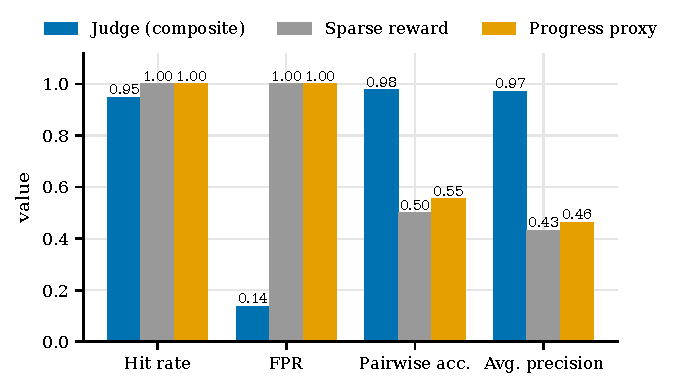
\includegraphics[width=0.62\linewidth]{fig-baseline-comparison.pdf}
\caption{Composite judge versus sparse-reward and progress baselines on the fresh capture's
held-out evaluation slice ($n{=}90$; source \texttt{summary-composite.json}). Both baselines
flag every prefix, so their hit rate and false positive rate are both 1.0; the judge trades
five points of hit rate for an 86-point false positive improvement, and the threshold-free
ranking metrics carry the calibration-fair comparison.}
\label{fig:baselines}
\end{figure}

\begin{figure}[t]
\centering
\begin{minipage}[t]{0.48\linewidth}
\centering
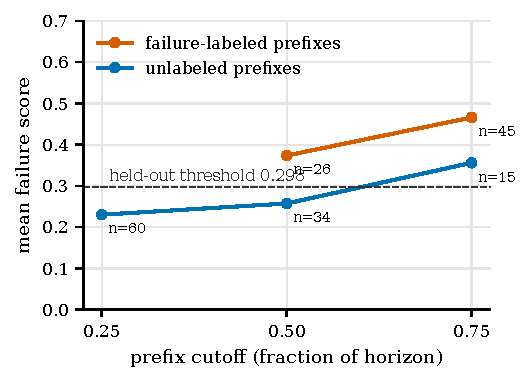
\includegraphics[width=\linewidth]{fig-early-separation.pdf}
\end{minipage}\hfill
\begin{minipage}[t]{0.48\linewidth}
\centering
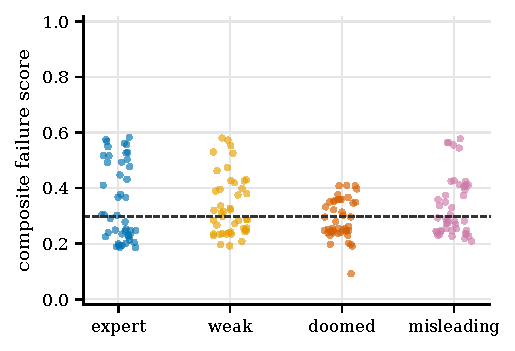
\includegraphics[width=\linewidth]{fig-score-distribution.pdf}
\end{minipage}
\caption{Left: mean composite failure score by cutoff on the fresh capture, split by the
heuristic prefix failure label. The labeler emits no failure label before cutoff 0.5 by
rule. Failure-labeled prefixes sit above the held-out threshold from the first cutoff at
which they exist; the unlabeled mean crosses it at cutoff 0.75, where four of the seven
false positives live (the other three sit marginally above threshold at cutoff 0.50).
Right: every composite failure score in the fresh capture by policy family (180 prefixes;
jitter is presentational). The families overlap substantially; the judge is not a family
classifier, and the held-out split is doing real work.}
\label{fig:separation}
\end{figure}

\begin{figure}[t]
\centering
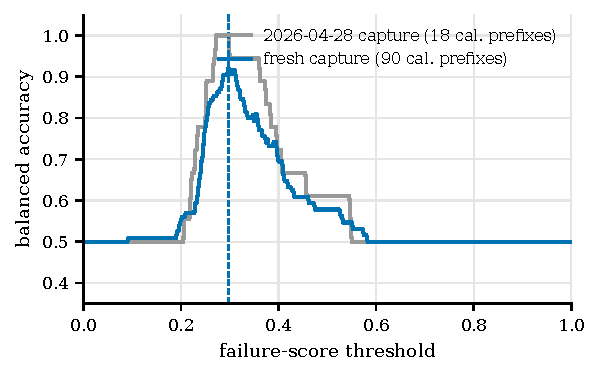
\includegraphics[width=0.6\linewidth]{fig-threshold-transfer.pdf}
\caption{Balanced accuracy over failure-score thresholds on the calibration cohorts (weak
and doomed families) of the two real captures, computed from the checked-in prefix and
judge files. Dashed lines mark each capture's selected threshold: 0.298006 (initial, grey)
and 0.297680 (fresh, blue). Disjoint captures recover the same operating point to within
$4\times10^{-4}$.}
\label{fig:transfer}
\end{figure}

The hybrid replay-time judge on the same fresh split scores a 0.923 hit rate, 0.137 false
positive rate, 0.976 pairwise accuracy, and 0.970 average precision at threshold 0.313437
(\judgemode{hybrid\_prefix\_latent\_judge}, \texttt{summary.json}). Consistent with
Section~\ref{sec:latent}, the latent term adds nothing over the composite here; its value,
if any, is in replay triage.

\subsection{Synthetic benchmark}
\label{sec:synthetic}

The synthetic slice (24 episodes, 72 prefixes, in-slice threshold 0.360053, failure-label
coverage 4 of 72) is the controlled proof surface: the generator constructs the failure
modes, so it isolates judge behavior from capture noise. The composite judge scores a 1.0
hit rate at 0.029 false positive rate with 0.985 pairwise accuracy; sparse reward again
ranks at chance (0.500) and the progress baseline ranks these families badly (0.147). The
threshold is in-slice and we report it as a debugging operating point, not an operating
claim. A held-out family split on synthetic data is degenerate by construction: the expert
and misleading evaluation families contain no failure-labeled prefixes there (synthetic
expert and weak episodes succeed by design, and synthetic misleading episodes stay
recoverable under the conservative labeler), so held-out evaluation metrics would honestly
return \texttt{null}, and the held-out story belongs to the real captures.

\subsection{How circular are the labels?}
\label{sec:circularity}

The labeler and the judge consume the same evidence family, so judge-versus-label agreement
is partly built in. We quantify the overlap instead of hand-waving it. Distance regret, the
single strongest shared feature, ranked with the same tie-handled pairwise statistic,
scores 0.985 on the synthetic slice, matching the judge's headline there; on real captures
it scores 0.825 (initial, $n{=}18$) and 0.824 (fresh, $n{=}90$) against the judge's 1.000
and 0.978. Three readings follow. First, on synthetic data the benchmark cannot distinguish
the composite from its strongest input, and synthetic separation should be discounted
accordingly. Second, on real captures the composite adds roughly fifteen points of pairwise
accuracy over its strongest single feature, so the aggregation is doing measurable work
beyond one input. Third, all of these comparisons remain within the shared evidence family;
labels independent of the judge's inputs (human annotation, or environment-defined failure
states) are the only way to close the question, and they are future work, not shipped.

\subsection{Reproducibility and cloud runs}
\label{sec:repro}

Every artifact directory carries the capture of record (\texttt{rollouts.jsonl}), every
derived table, both judge outputs, both summaries, and rendered reports; deterministic
stages regenerate byte-identically on the pinned interpreter (CPython 3.11). The fresh
capture reported here was executed end to end on Hugging Face Jobs CPU hardware: the
launcher refuses dirty or unpushed working trees, pins the remote installation to the exact
commit under review, and gates the published run folder against a 22-check contract
(checksums of every file, row-count joins, \judgemode{judge\_mode} values, and calibration
provenance) before it can be cited. The full pipeline for the 60-episode capture took 24.7
seconds of stage wall time; the run's \texttt{provenance.json} records the argv, timing,
and SHA-256 of every stage and file, and the published copy is public.\footnote{Run
\texttt{metaworld-benchmark-20260713-080743-g666670e} under
\url{https://huggingface.co/datasets/abdelstark/leworldmodel-judge-runs}.} Total compute
cost for the full run matrix was under one cent, which we mention not as an efficiency
claim but as evidence that nothing about the benchmark requires trust in unreproducible
infrastructure.

\section{Limitations}
\label{sec:limitations}

\textbf{The slices are small and narrow.} Ninety held-out evaluation prefixes from sixty
episodes across three tasks in one simulator is enough to falsify perfect separation and
measure a ranking gap; it is not enough to support claims about manipulation in general,
other simulators, or real robots, and we make none.

\textbf{The labels are heuristics over the judge's own evidence family.}
Section~\ref{sec:circularity} bounds the overlap but cannot eliminate it. Worse, in both
real captures no episode reaches terminal success within the 75-step cap, so the
environment-truth veto never fires on real data and every real-data metric rests on the
heuristic labels. The honest reading of Table~\ref{tab:heldout} is therefore: the judge
ranks prefixes by imminent failure as a conservative task-aware labeler defines it,
substantially better than sparse reward does, under thresholds that transfer across
captures. Whether that ordering matches human judgment of doom is unmeasured.

\textbf{The judge is a hand-weighted heuristic and the latent proxy is not a world model.}
No learned encoder, no trained dynamics, no representation learning of any kind ships in
these results. The project's name states its research program, not its implementation
status, and the per-row \judgemode{judge\_mode} tags exist precisely so the two cannot be
confused. The hybrid variant is additionally replay-time only.

\textbf{Detection is not the judge's win on these slices; nor is lead time measured.} Both
baselines reach hit rate 1.0 by flagging everything, so the win is false positives and
ranking. Metrics pool the three cutoffs; "early" is structural (labels and scores exist at
fixed early cutoffs) rather than a measured detection lead time, and per-cutoff lead-time
analysis is future work.

\textbf{Calibration is asymmetric.} Only the judge threshold is calibrated; the progress
baseline keeps a fixed default and sparse reward is binary. The threshold-free rows are the
fair comparison, and they are the rows the conclusions rest on.

\section{Conclusion}
\label{sec:conclusion}

We set out to test a narrow proposition: that a world-model-motivated, fully auditable
surprise signal can judge partial manipulation rollouts earlier and more usefully than
sparse reward, under an evaluation protocol that states the provenance of every threshold
and measures the circularity it cannot remove. On the locked slice the proposition survives contact with a fresh capture: the
ranking gap over sparse reward persists at five times the evaluation cohort, the calibrated
threshold transfers across disjoint captures, and the places where the judge degrades are
identifiable in the released files down to individual prefixes. The protocol contributions
(family-held-out threshold calibration with mandatory provenance, per-row judge-mode tags,
the cutoff-time versus replay-time boundary, and a verify-gated artifact contract) are
independent of the current heuristic judge and are, we think, the durable part of this
work. The obvious next step is the one the project's name promises: replace the mean-pooled
observation proxy with a learned encoder and a continuation predictor that is computable at
the cutoff, then hold it to the same benchmark, the same provenance rules, and the same
willingness to publish degradation.

\subsection*{Acknowledgments}

The cloud execution path runs on Hugging Face Jobs, and parts of the operational tooling
were exercised by Hugging Face's ml-intern agent under scoped prompts, with transcripts
published alongside the runs. All analysis, claims, and errors are the author's.

\bibliographystyle{plainnat}
\bibliography{references}

\appendix

\section{Reproduction commands}
\label{app:repro}

The pipeline is a single CLI (\texttt{lewm-judge}, or \texttt{python -m leworldmodel\_judge})
with one subcommand per stage. The fresh capture reported in Section~\ref{sec:heldout}
regenerates its derived files from the checked-in capture of record:

\begin{small}
\begin{verbatim}
RUN=artifacts/hard-family-real-fresh-capture-2026-07-13
lewm-judge prefixes  --input $RUN/rollouts.jsonl --output $RUN/prefixes.jsonl
lewm-judge latents   --rollouts $RUN/rollouts.jsonl \
                     --prefixes $RUN/prefixes.jsonl \
                     --output $RUN/latent-cache.jsonl
lewm-judge baselines --input $RUN/prefixes.jsonl --output $RUN/baselines.jsonl
lewm-judge judge     --input $RUN/prefixes.jsonl --mode heuristic_surprise \
                     --output $RUN/judge-composite.jsonl
lewm-judge judge     --input $RUN/prefixes.jsonl --mode hybrid_surprise \
                     --latent-cache $RUN/latent-cache.jsonl \
                     --output $RUN/judge-hybrid.jsonl
lewm-judge evaluate  --prefixes $RUN/prefixes.jsonl \
                     --baselines $RUN/baselines.jsonl \
                     --judge $RUN/judge-composite.jsonl \
                     --calibration-families weak,doomed \
                     --evaluation-families expert,misleading \
                     --output $RUN/summary-composite.json
\end{verbatim}
\end{small}

The capture itself was collected on Hugging Face Jobs with the repository launcher
(\texttt{uv run jobs/launch.py launch --preset metaworld-benchmark}), which is equivalent to
\texttt{lewm-judge collect --source metaworld --task all --episodes 5 --max-steps 75 --seed
1013 --policy-family expert,weak,doomed,misleading} followed by the chain above. Meta-World
capture is not byte-reproducible across simulator builds; rerunning reproduces the protocol,
not the bytes, which is why the capture is checked in.

Every figure in this paper regenerates from the checked-in artifacts with
\texttt{uv run docs/paper/figures/make\_figures.py}, and the paper builds with
\texttt{make -C docs/paper}.

\end{document}
